\section{Filter}\hartl{509}
\subsection{Inhaltsverzeichnis}
\begin{itemize}
  \item Aufgaben von Filtern
  \item Implementation von passiven Filtern
  \item Implementation von aktiven Filtern
\end{itemize}

\subsection{Aufgaben von Filtern, Verstärkern}
\begin{itemize}
  \item Unterdrückung von störenden Frequenzen im Signal
  \item Verstärkung von "`gewünschten"' Frequenzen
  \item Begrenzung der Bandbreite
  \begin{itemize}
    \item Anti-Aliasing Filter
    \item Noise-Reduktion
  \end{itemize}
  \item Signalanpassung an ADC-Eingangs-Spannungsbereich
\end{itemize}
\newpage
\subsection{Tiefpass-Filter}\hartl{514}

\subsubsection{1. Ordnung}
\begin{itemize}
  \item Aufbau\\
  \begin{figure}[htb]
  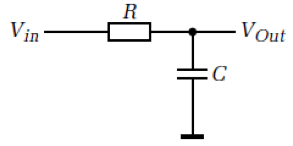
\includegraphics[scale=0.4]{pictures/tiefpass1ordnung}
  \end{figure}
  \item Übertragungsfunktion 
  \begin{equation}
  G1(s)=\frac{1}{1+s*C*R}
  \end{equation}
  \item Zeitkonstante T\\
  Bei $j\omega=\frac{1}{T}$sin Real-  und Imaginärteil gleich gross
  \begin{equation}
  T:=\frac{1}{R*C}
  \end{equation}
  \item $\to$ Amplitude $\frac{1}{1.41}\to 3dB$
  \begin{equation}
  f_{3dB}=\frac{1}{2\pi R*C}
  \end{equation}
  \item Amplitudengang (3dB bei 1kHz)\\
  \begin{figure}[!htbs]
  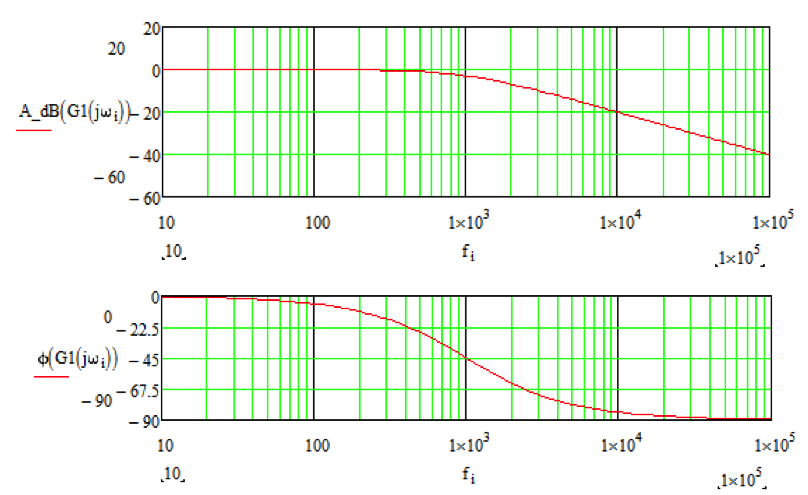
\includegraphics[scale=0.5]{pictures/tiefpass1ordnungamplitude}
  \end{figure}
  
\end{itemize}
\newpage
\subsubsection{2. Ordnung}
\begin{itemize}
  \item Kaskadierte RC-Tiefpässe\\
  \begin{figure}[htb]
  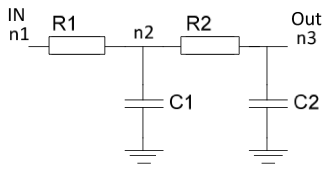
\includegraphics[scale=0.4]{pictures/tiefpass2ordnung}
  \end{figure}
  \item Stromgleichungen für Knoten n2 und n3 (out)
  \begin{gather}
  0=(u2-Uin)*\frac{1}{R1}+(U2-U3)*\frac{1}{R2}+U2*s*C1\\
  0=(U3-U2)*\frac{1}{R2}+U3*s*C2\\
  U2=R2*U3*(\frac{1}{R2}+s*C2)\\
  \text{U2 in oberer Gleichung eingesetzt und aufgelöst für U*/Uin}\notag\\
  G_{p}(s)=\frac{1}{C1*R1*s+C2*R1*s+C2*R2*s+C1*C2*R1*R2*s^2+1}
  \end{gather}
  Vergleich: Allgemeine Beschreibung von Tiefpass 2. Ordnung mit
  Verstärkung A0, Kreisfrequenz $\omega_{0}$ und Güte Q
  \begin{gather}
  T_{lp}(s)=\frac{A0}{\frac{s^2}{\omega_{0}^2}+\frac{s}{Q\omega_{0}}+1}\\
  A0=1\notag\\
  \omega_{0}=\frac{1}{\sqrt{C1*C2*R1*R2}}\\
  \text{Güte berechnet mit Termen, die s enthalten}\notag\\
  \frac{s}{Q*\omega_{0}}=C1*R1*s+C2*R1*s+C2*R2*s\\
  Q:=\frac{\sqrt{C1*C2*R1*R2}}{R1*(C1+C2)+C2R2}
  \end{gather}
  Passive RC-Filter können maximal Güte von 0.5 haben (2 identische reelle
  Pole) Filter höherer Güte benötigen Spulen oder Verstärker
\end{itemize}
\newpage
\subsection{Sallen Key (Einfachmitkopplung)}\hartl{517}
\begin{figure}[htb]
\centering
 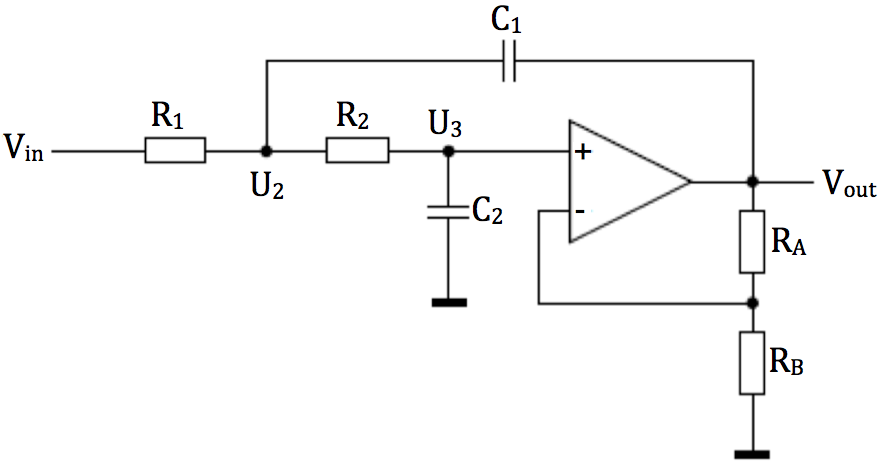
\includegraphics[scale=0.5]{pictures/sallenkey}
\end{figure}
\begin{gather}
0=(U2-Uin)*\frac{1}{R1}+(U2-U3)*\frac{1}{R2}+(U2-Uout)*s*C1\\
0=(U3-U2)*\frac{1}{R2}+U3*s*C2\\
\text{Opamp: }Uout=G0*U3\\
G0=\frac{R_{A}+R_{B}}{R_{B}}\\
G_{SK}(s):=\frac{G0}{C1*C2*R1*R2*s^s+s*[C2*(R1+R2)+C1*R1*(1-G0)]}+1\\
\text{Güte: }Q_{SK}(G0)=\frac{\sqrt{C1*C2*R1*R2}}{C2*(R1+R2)+C1*R1*(1-G0)}
\end{gather}
\subsubsection{Sallen Key-Filter bei hohen Frequenzen}
\begin{figure}[htb]
\centering
 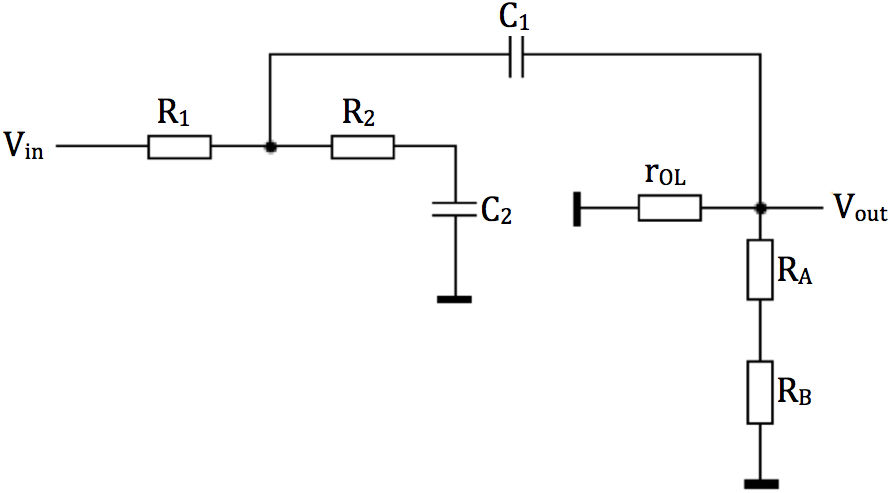
\includegraphics[scale=0.5]{pictures/sallenkey2}
\end{figure}
\begin{itemize}
  \item Wenn der Opamp nicht mehr verstärkt
  \item C1, C2 wirken wie Kurzschlüsse
  \begin{equation}
  \frac{V_{Out}}{V_{in}}=\frac{r_{OL}\parallel R2\parallel
  (R_{A}+R_{B})}{R1+r_{OL}\parallel R2\parallel (R_{A}+R_{B})}\approx
  \frac{r_{OL}}{R1+r_{OL}}
  \end{equation}
  \item Folge: Sallen Key-Filter sind nicht geeignet für Systeme mit hohen
  Frequenzanteilen, z.B. PEM-DAC
\end{itemize}
\newpage
\subsection{Multiple Feedback}\hartl{522}
\begin{figure}[!h]
\centering
 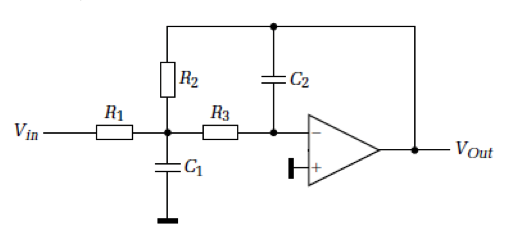
\includegraphics[scale=0.5]{pictures/mulipleFeedback}
\end{figure}
\begin{gather}
0=(U2-Uin)*\frac{1}{R1}+(U2-Uout)*\frac{1}{R2}+(U2-U3)*\frac{1}{R3}+U2*s*C1\\
0=(U3-U2)*\frac{1}{R3}+(U3-Uout)*s*C2\\
\text{Opamp sorg für }U3=0\notag\\
G_{mf}(s)=\frac{G0}{1+C2(R2+R3+R3*\frac{R2}{R1})*s+C1*C2*R2*R3*s^s}\\
Q_{mf}=\frac{\sqrt{C1*C2*R2*R3}}{C2*(R2+R3+R3*\frac{R2}{R1})}
\end{gather}
Die Güte wird v.a. eingestellt mit C2 und R1, grosse Güte für kleines C2 und
grosses R1. C2 beeinflusst auch das Frequenzverhalten, R1 die Verstärkung.
\newpage
\subsection{Zustandsvariablen-Filter}
\begin{figure}[!h]
\centering
 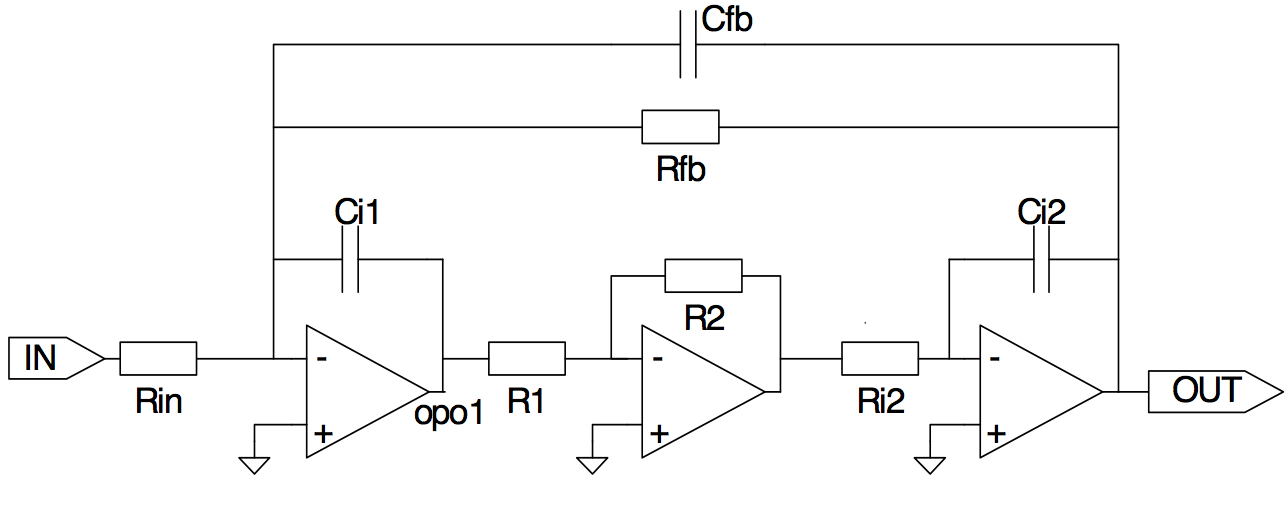
\includegraphics[scale=0.5]{pictures/zustandsvariable}
\end{figure}
\begin{gather}
V{out}=-\frac{1}{s*Ci2*Ri1}*V_{opo2}\\
V_{opo2}=-\frac{R2}{R1}*V_{opo1}\\
V_{opo1}=\frac{-1}{s*Ci1}*(\frac{V_{in}}{R_{in}}+\frac{V_{out}}{Rfb}+s*Cfb*V_{out})\\
G_{ss}(s)=\frac{-\frac{Rfb}{rin}}{Ci1*Ci2*Ri1*Rfb*\frac{R1}{R2}*s^2+Cfb*Rfb*s+1}\\
\omega_{0}=\frac{1}{\sqrt{Ci1*Ci2*Ri1*Rfb*\frac{R1}{R2}}}\\
A0=-\frac{Rfb}{Rin}\\
Q=\frac{\sqrt{Ci1*Ci2*Ri1*Rfb*\frac{R1}{R2}}}{Cfb*Rfb}
\end{gather}
D.h. mit dieser Topologie sind alle 3 Parameter frei wählbar!
\begin{enumerate}
  \item $\omega_{0}$ mit Ci1, Ci2, Rfb, Ri2, R1, R2
  \item Q mit Cfb
  \item A0 mit Rin
\end{enumerate}

\subsection{Zusammenfassung}
\begin{itemize}
  \item Filter dienen der
  \begin{itemize}
    \item Unterdrückung von störenden Frequenzen im Signal
    \item Verstärkung von "`gewünschten"' Frequenzen
    \item Begrenzung der Bandbreite
   \end{itemize}
   \item Aktive Filter sind nötig für Polgüten $>0.5$
   \item Filterschaltungen können gleichzeitig zur Signalanpassung an
   ADC-Eingangs-Spannungsbereich verwendet werden
\end{itemize}


